\documentclass{szzclass}

\title{Nástroje pro podporu tvorby softwarových produktů: Sledování chyb a správa úkolů (používané nástroje, typický životní cyklus úkolu/chyby),
 správa a sdílení zdrojových kódů (principy řešení spolupráce, hlavní přínosy, používané nástroje).}
\author{Jakub Rathouský}

\begin{document}
\maketitle
\newpage
\tableofcontents
\newpage

\section{Správa úkolů, požadavků, chyb}
Pomáhá vyřešit organizaci práce v týmu
\begin{itemize}
    \item evidence úkolů - co je nutné udělat
    \item přidělování - kdo to bude dělat
    \item plánování - do kdy je nutné úkol udělat
    \item kontrola splnění úkolů
    \item vyhodnocení odvedené práce
\end{itemize}
\subsection{Používané nástroje}
\begin{itemize}
    \item Trac tickets
    \item Mantis
    \item Bugzilla
    \item JIRA
    \item GitLab/Github
    \item Redmine
    \item Youtrack
\end{itemize}
\subsection{Typický životní cyklus úkolu/chyby}
Kroky:
\begin{itemize}
    \item Team leader/project manager vyvoří úkol/nahlášení chyby $\rightarrow$ stav \textit{\textbf{Nový(New)}}
    \item přiřazení úkolu řešiteli (Team leader), převzetí úkolu řešitelem $\rightarrow$ stav \textit{\textbf{Přiřazemý(Assigned)}}
    \item dokončení úkolu $\rightarrow$ stav \textit{\textbf{Vyřešený(Resolved)}}
    \begin{itemize}
        \item reportér nesouhlasí s řešením $\rightarrow$ stav \textit{\textbf{Znovuotevřený(Reopen)}}
        \begin{itemize}
            \item dokončení úkolu $\rightarrow$ stav \textit{\textbf{Vyřešený(Resolved)}}
            \item nebo přiřazení úkolu jinému řešiteli $\rightarrow$ stav \textit{\textbf{Přiřazený(Assigned)}}
        \end{itemize}
        \item nebo potvrzení vyřešení reportérem $\rightarrow$ stav \textit{\textbf{Uzavřený(Closed)}}
    \end{itemize}
\end{itemize}
\begin{figure}
    \centering
    % \includegraphics[width=1.3\textwidth]{images/cycle.png}
    \includegraphics[width=1\textwidth]{topics/bi-spol-30/images/cycle.png}
\end{figure}
\newpage
\section{Sdílení a správa souborů}
\subsection{Hlavní přínosy}
Řeší více dílčích problémů
\begin{itemize}
    \item verzování
    \begin{itemize}
        \item udržuje kompletní historii každého souberu pod správnou verzí
        \item lzde se k jednotlivým verzím v minulosti kdykoliv vrátit
    \end{itemize}
    \item zálohování
    \begin{itemize}
        \item v případě poškození/ztráty souborů je možné je obnovit
    \end{itemize}
\end{itemize}
\subsection{Používané nástroje}
\begin{itemize}
    \item centralizované
    \begin{itemize}
        \item SVN
        \item CVS
    \end{itemize}
    \item distribuované
    \begin{itemize}
        \item GIT
        \item Mercurial
    \end{itemize}
\end{itemize}
\subsubsection{Centralizované nástroje}
\begin{itemize}
    \item veškeré revize/verze souborů jsou uloženy pouze v centrálním repozitáři
    \item na lokálním počítači je pouze pracovní kopie (aktuální revize/verze) souborů
\end{itemize}
\subsubsection{Distribuované nástroje}
\begin{itemize}
    \item na lokálním počítači jsou uloženy všechny revize/verze
    \item díky tomu může být velká část operací prováděna lokálně
\end{itemize}
\subsection{Principy řešení spolupráce}
Dělí se na dva principy
\begin{itemize}
    \item zamknutí - úprava - odemknutí (lock - modify - unlock) $\rightarrow$ pouze centralizované systémy
    \item kopie - úprava - sloužení (copy - modify - merge) $\rightarrow$ centralizované i distribuované systémy
\end{itemize}
\subsubsection{zamknutí - úprava - odemknutí}
\begin{itemize}
    \item může způsobit organizační problém
    \begin{itemize}
        \item zbytečně blokovaní práce uživatelů při zapomenutí odemknutí po dokončení práce
        \item nutnost násilného uvolnění zámku, které může způsobit ztrátu odvedené práce
    \end{itemize}
    \item vynucuje serializovaný přístup i při nekonfliktních úpravách
    \item využítí pro soubory, které nelze po částech sloučit (grafika, modely...)
\end{itemize}
\subsubsection{kopie - úprava - sloužení}
\begin{itemize}
    \item častěji využívaný způsob spolupráce
    \item odstaňuje problémy zamykacího režimu
    \item v případě konfliktních změn je nutné provést ruřně sloučení
\end{itemize}
\end{document}